\section{Chronic Disease Surveillance}
\label{c1:sec:invasive_tests}
Non-communicable diseases (NCDs) such as cancer, diabetes, cardiovascular, and respiratory diseases are a 21st-century global pandemic. They affect men and women equally and cause 60\% to 70\% of all human deaths worldwide~\citep{world2014global, bennett2018ncd}. Often NCDs are chronic. Hence, in many \emph{low-risk} NCD diagnoses (e.g., localized prostate cancer, low-risk dysplasia), immediate serious treatments like surgery, radiotherapy, etc., can induce side-effects and reduce a patient's overall quality of life. A common alternative to immediate treatment is delaying it until the disease has \emph{progressed}, a curable non-terminal disease stage. In this regard, monitoring patients for progression, with curative intent, is called \emph{surveillance}. 

The goal of surveillance is to timely detect progression, upon which patients are typically removed and treated. However, the transition of a patient's \emph{disease state} from low-risk to progressed disease is not directly observable. Instead, auxiliary modalities such as biomarkers, physical examinations, medical imaging, biopsies, etc., are used to determine the disease state. Among these, the gold standard \emph{tests} for confirming progression are typically \emph{invasive} (e.g., biopsies). For timely observing the occurrence of progression, invasive tests are conducted repeatedly in surveillance. For example, biopsies are the benchmark test for verifying progression in surveillance of localized prostate cancer~\citep{bokhorst2015compliance}. Similarly, endoscopies are utilized in Barrett's esophagus~\citep{choi2012screening} and colonoscopies in colorectal cancer~\citep{krist2007timing} surveillance. Repeat bronchoscopies, and core biopsies are also employed to detect allograft deterioration in lung~\citep{mcwilliams2008surveillance} and kidney transplant~\citep{henderson2011surveillance} patients, respectively.

\subsection{Invasive Test: Burden versus Benefit}
Currently, repeated invasive tests are a necessary \emph{burden} for patients. They are indispensable for confirming progression, but they are also difficult to perform, may cause pain, and can lead to severe complications~\citep{loeb2013systematic,krist2007timing}. Consequently, invasive tests are usually planned with a considerable time gap between them. For example, in prostate cancer surveillance, it is recommended to maintain a time difference of one year between consecutive biopsies. However, a time gap between tests also leads to a \emph{time delay} in detecting progression (Figure~\ref{c1:fig:1}). When tests are conducted periodically, this delay can be reduced by scheduling tests frequently. The argument for lowering delay is that detecting progression earlier may provide a larger window of opportunity for curative treatment. Also, timely treatment may also have an impact on the patient's (quality-adjusted) life-years remaining. Hence, a balance between the number and frequency of tests (burden) and time delay in detecting progression (shorter is beneficial) is of crucial importance for patients.

\begin{figure}[tbp]
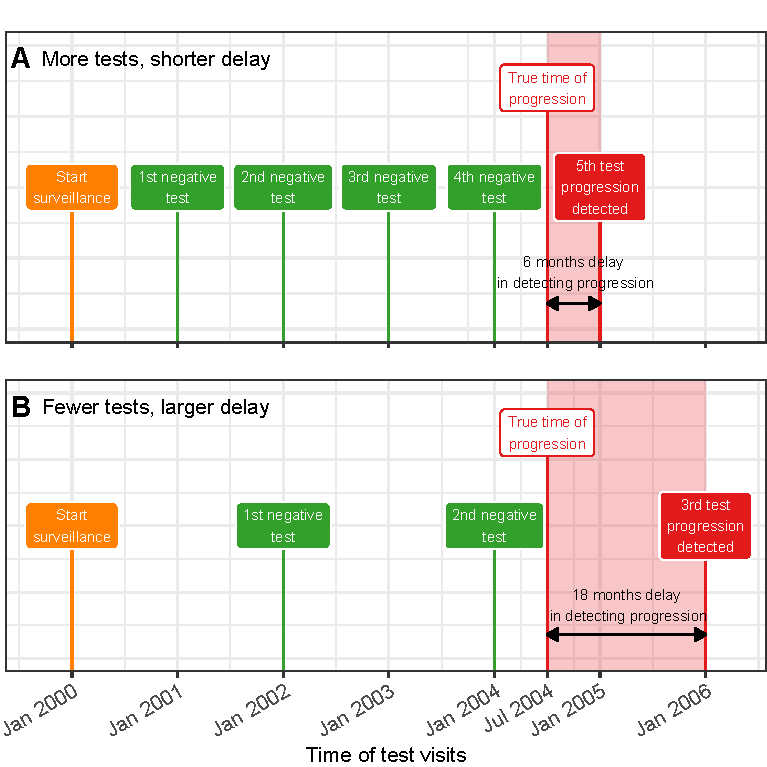
\includegraphics{contents/c1/images/c1_fig1.pdf}
\caption{\textbf{Trade-off between the test frequency and the time delay in detecting disease \emph{progression}:} The true time of disease progression for the patient in this figure is July 2008. More frequent tests in \textbf{Panel~A}, lead to a shorter time delay in detecting progression, than fewer tests in \textbf{Panel~B}. Due to the periodical nature of tests, the time of progression is always observed as an interval. For example, between Jan~2004--Jan~2005 in \textbf{Panel~A} and between Jan~2004--Jan~2006 in \textbf{Panel~B}.}
\label{c1:fig:1}
\end{figure}

\subsection{Schedules for Invasive Tests}
\label{c1:subsec:scheduling_methodologies}
The frequency of invasive tests varies across diseases and cohorts. However, within a cohort, usually a constant frequency or \emph{fixed schedule} (e.g., every six months) is employed for all patients~\citep{henderson2011surveillance,bokhorst2015compliance,krist2007timing}. The primary drawback of a fixed schedule is its \emph{one-size-fits-all} assumption. Specifically, high-frequency tests promise shorter delays in detecting progression at the cost of imposing an extra burden on patients who progress slowly and/or patients who never experience progression (e.g., due to comorbidities). The vice versa holds for infrequent tests. Schedules with a skewed burden benefit ratio are also prone to patient non-compliance~\citep{bokhorst2015compliance,LeClercq2015325}. Reduced compliance for invasive tests may lead to the original problem of delayed detection of disease progression, and reduce the effectiveness of surveillance. 

Several improvements have been proposed over one-size-fits-all fixed schedules. The underlying methodology of these advances can be broadly divided into three categories. Namely, sub-group specific fixed schedules, schedules cost-optimized using Markov decision processes, and schedules optimizing a specific utility function of the clinical parameters of interest. Two commonly used terms across these three methodologies are \emph{personalized/individualized/tailored} schedules, and \emph{optimal} schedules. Loosely, personalization means a unique schedule for each patient in a study population. Optimal refers to mathematical optimization of certain schedule-specific criteria to automatically derive a schedule.

\paragraph{Sub-group specific fixed schedules}
These schedules are typically prescribed based on observed patient data such as biomarkers, physical examinations, medical imaging, or previous test results. For example, in Barrett's esophagus patients observing low-risk dysplasia on a repeat endoscopy are prescribed future endoscopies every six to twelve months, rather than the standard once every three to five years~\citep{choi2012screening}. Sub-groups are also formed based on multiple results. For example, in the world's largest prostate cancer surveillance PRIAS, the time of biopsies is decided using observed \emph{prostate-specific antigen (PSA)} value, the average rate of change of PSA, the size and shape of the tumor, and previous biopsy results (Figure~\ref{c1:fig:c1_prias_biopsy_protocol}). There are two main shortcomings of such heuristic schedules. First, they often create sub-groups based on observed data without accounting for ascertainment biases and measurement error. Second, as illustrated in Figure~\ref{c1:fig:c1_prias_biopsy_protocol}, instead of utilizing complete observed data, they typically use only the latest observed value, that too after categorizing continuous ones.

\begin{figure}[tbp]
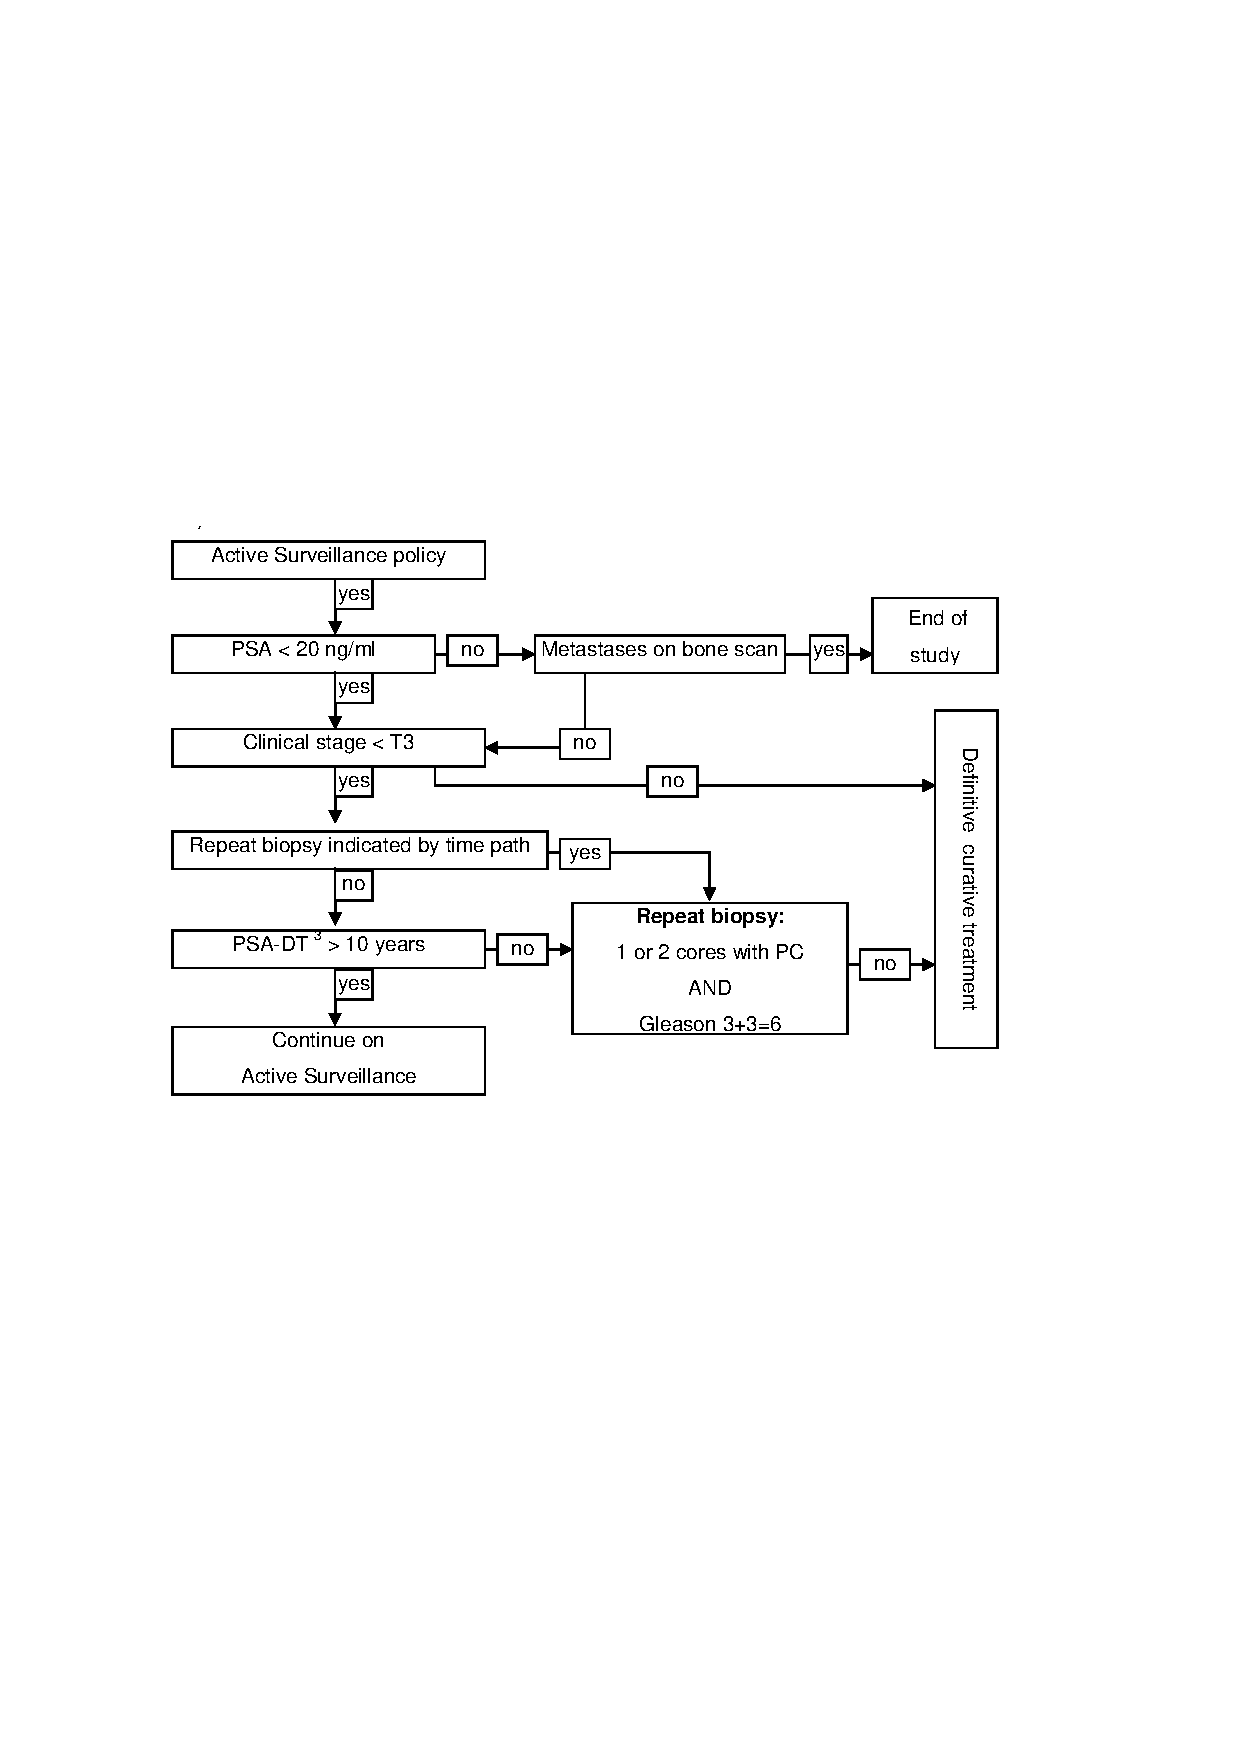
\includegraphics{contents/c1/images/c1_prias_biopsy_protocol.pdf}
\caption{\textbf{Treatment and biopsy protocol} of the world's largest localized prostate cancer surveillance program PRIAS. Source:~\url{https://www.prias-project.org}}
\label{c1:fig:c1_prias_biopsy_protocol}
\end{figure}

\paragraph{Partially observable Markov decision processes} or POMDPs have been utilized in numerous optimal screening and surveillance test schedules for chronic diseases~\citep{steimle2017markov,denton2018optimization}, and especially for nearly all types of cancers~\citep{alagoz2010operations}. A notable advantage of POMDPs is that they find an optimal schedule from all schedules possible over a set of follow-up visits. The criterion of optimality in POMDPs is the weighted cumulative reward. A reward is a number that is chosen manually for four possible outcomes (true-positive, false-positive, true-negative, and false-negative) of a binary test/no test decision in a schedule. The weighted cumulative reward of a schedule is the weighted sum of all rewards possible with all sequential test decisions in a schedule. The weights are probabilities from a joint probability distribution of the disease state of the patient and the auxiliary outcomes (e.g., biomarkers) that manifest this state. This joint distribution is allowed to change over time.

In general, POMDP algorithms suffer from the curse of dimensionality if continuous longitudinal outcomes or continuous time-space is used~\citep{sunberg2018online}. However, a more substantial drawback of POMDPs is their very flexible specification. Specifically, in a simple POMDP with binary test/no test decisions, and binary disease state (low-risk, progressed), it can be shown that there exist infinite possible rewards result in the same optimal schedule (Chapter~\ref{c4:appendix:pomdp}). Typically POMDP rewards are chosen based on survey results~\citep{denton2018optimization} and translated as quality-adjusted life-years saved. However, with infinite optimal reward sets, any reward set can be cherry-picked, including those that correspond to (improbable) thousands of quality-adjusted life-years saved. Last, to our knowledge, POMDPs are not currently personalized. Since they exploit population-level joint distributions of disease state (e.g., Kaplan-Meier curve) and auxiliary outcomes, the resulting schedules are not personalized.

\paragraph{Schedules optimized for clinical parameters of interest} An option to the POMDP framework is optimizing a utility function of the clinical parameters of interest directly~\citep{bebu2018optimal,parmigiani1996optimal}. Examples of clinical parameters are, namely, the financial cost for treating progression, reduction in lifespan due to delayed detection of progression, cost of invasive tests, reduction in quality of life due to invasive tests. Others have proposed optimizing test decision rules for the corresponding sensitivity and specificities in detecting progression~\citep{wang2019learning}. Alternatively, one may optimize information-theoretic measures such as Wasserstein distance~\citep{hanin2001optimal} or Kullback-Leibler divergence~\citep{rizopoulos2016personalized} between the disease state probability distribution at the beginning of surveillance and at a future time point. 

In all of these approaches, the expected utility is calculated using the probability distribution of the disease state of the patient. It is standard to use a time-varying disease state distribution. Although, this distribution can be either discrete (e.g., a Markov model with low-risk, medium-risk, progressed disease states) or continuous (e.g., Cox model).

\subsection{Goal: Developing Personalized Schedules}
\label{c1:subsec:goal}
The overall aim of this work was to develop personalized schedules that better balance the overall burden and benefit of repeated invasive tests in surveillance than one-size-fits-all fixed schedules. The subgoals and specific research questions that we intend to answer in this work are as follows.
\begin{itemize}
  \item To find a suitable statistical modeling framework to process observed patient data. 
  \item Evaluating the efficacy of different utility functions while planning tests by optimizing clinical parameters of interest (e.g., time delay in detecting progression).
  \item Evaluating the pros and cons of the widely used POMDP framework for scheduling tests.
  \item How to schedule invasive tests based on a patient's risk of progression?
  \item On which criteria should patients chose a personalized schedule over a fixed schedule and vice versa?
  \item Which factors (e.g., cohort, type of disease) affect the performance of a personalized schedule?
  \item Can the same test scheduling framework be used across different cohorts and diseases?
\end{itemize}
To answer our research questions and to develop personalized schedules, the process we followed consisted of four steps. First, processing the observed data of the patient. For example, directly using data via flowcharts (Figure~\ref{c1:fig:c1_prias_biopsy_protocol}), using summary statistics, and statistical modeling of observed data, etc. Second, choosing the reward/utility/loss function and the corresponding clinical parameters. Third, defining criteria and methodology for comparing proposed personalized schedules with currently practiced schedules. Fourth, implementing personalized schedules in a computer application for practitioners. 

\paragraph{Processing observed data} In surveillance, observed data consists of baseline patient characteristics, longitudinally measured outcomes, and previous invasive test results. Since all of these manifest the underlying disease state of the patient, they are usually correlated as well. To accommodate outcomes of various types, we utilized the framework of joint models for time-to-event and longitudinal data~\citep{rizopoulos2012joint, tsiatis2004joint}. The motivation of this choice was that joint models combine observed data into a patient-specific cumulative-risk of progression over the entire follow-up period. This risk profile manifests the underlying latent disease state of the patient.

\paragraph{Choosing of reward/utility/loss function and clinical parameters of interest} Once a risk profile for progression is available, the next step is to utilize it for optimizing clinical parameters of interest. Examples of these parameters are the time of disease progression, time delay in detecting disease progression given a schedule (Figure~\ref{c1:fig:1}), number and timing of tests in a schedule, cumulative-risk of disease progression, sensitivity/specificity of an invasive test and their derivatives such as Youden index and F1score~\citep{lopez2014optimalcutpoints}. We optimized these parameters via both standard utility functions such as squared loss, absolute loss, multilinear loss~\citep{robertBayesianChoice}, and custom utility functions that are a linear sum of multiple clinical parameters of interest.

\paragraph{Comparing personalized versus fixed schedules} There are no single perfect criteria to compare schedules. Some important ones, though, are how many patient deaths and/or progression to an advanced disease state (e.g., metastasis) are saved. Reliable data on such metrics are difficult to obtain in low-grade diseases. This is because, in such diseases, the prevalence of death from disease can be quite low (e.g., almost zero in low-grade prostate cancer active surveillance). Hence in this work, we used two other criteria for comparing the performance of proposed personalized schedules with existing fixed schedules; Specifically, the number and timing of invasive tests (burden of tests) and time delay in the detecting progression (shorter is beneficial). Our choice of these criteria is motivated by two reasons. First, we argue that time delay in detection of progression is an easily-quantifiable surrogate for important clinical aspects such as the window of opportunity for curative treatment, risk of adverse downstream outcomes, quality-adjusted remaining lifetime, and additional complications in treating a delayed progression. Similarly, the number and timing of tests manifest financial costs of tests, risk of side-effects, and reduction in quality of life, etc. Second, both the number of tests and time delay in detecting progression are easy to understand for both patients/doctors and can better facilitate \emph{shared decision making} of test schedules.

\paragraph{Computer application implementing personalized schedules} While there is no lack of existing methodologies for making invasive test schedules, presenting them in a user-friendly computer/web/phone application may increase their awareness and/or adoption. In this regard, we implemented personalized schedules in a web-application for real patients of the seven largest prostate cancer active surveillance programs. Also, we provide our scheduling methodology as a generic R application programming interface for surveillance of other diseases.